%%%%%%%%%%%%%%%%%%%%%%%%%%%%%%%%%%%%%%%%%
% Make sure to set your name, legi number and url to the right git branch.
\newcommand{\hmwkAuthorName}{Robin Spiess} % Your name
\newcommand{\hmwkAuthorLegi}{12-915-302} % Your name
\newcommand{\hmwkGitBranch}{12-915-302/1\_locally\_linear\_embedding} % Your name
%
%%%%%%%%%%%%%%%%%%%%%%%%%%%%%%%%%%%%%%%%%

%----------------------------------------------------------------------------------------
%	PACKAGES AND OTHER DOCUMENT CONFIGURATIONS
%	Skip this
%----------------------------------------------------------------------------------------

\documentclass{article}

\usepackage{fancyhdr} % Required for custom headers
\usepackage{lastpage} % Required to determine the last page for the footer
\usepackage{extramarks} % Required for headers and footers
\usepackage{graphicx} % Required to insert images
\usepackage{lipsum} % Used for inserting dummy 'Lorem ipsum' text into the template

\usepackage{amsmath}
\usepackage{graphicx}

% Margins
\topmargin=-0.45in
\evensidemargin=0in
\oddsidemargin=0in
\textwidth=6.5in
\textheight=9.0in
\headsep=0.25in 

\linespread{1.1} % Line spacing

% Set up the header and footer
\pagestyle{fancy}
\lhead{\hmwkAuthorName} % Top left header
\chead{\hmwkClass\ \hmwkTitle} % Top center header
\rhead{\firstxmark} % Top right header
\lfoot{\lastxmark} % Bottom left footer
\cfoot{} % Bottom center footer
\rfoot{Page\ \thepage\ of\ \pageref{LastPage}} % Bottom right footer
\renewcommand\headrulewidth{0.4pt} % Size of the header rule
\renewcommand\footrulewidth{0.4pt} % Size of the footer rule

\setlength\parindent{0pt} % Removes all indentation from paragraphs

%----------------------------------------------------------------------------------------
%	DOCUMENT STRUCTURE COMMANDS
%	Skip this
%----------------------------------------------------------------------------------------

% Header and footer for when a page split occurs within a problem environment
\newcommand{\enterProblemHeader}[1]{
\nobreak\extramarks{#1}{#1 continued on next page\ldots}\nobreak
\nobreak\extramarks{#1 (continued)}{#1 continued on next page\ldots}\nobreak
}

% Header and footer for when a page split occurs between problem environments
\newcommand{\exitProblemHeader}[1]{
\nobreak\extramarks{#1 (continued)}{#1 continued on next page\ldots}\nobreak
\nobreak\extramarks{#1}{}\nobreak
}

\setcounter{secnumdepth}{0} % Removes default section numbers
\newcounter{homeworkProblemCounter} % Creates a counter to keep track of the number of problems

\newcommand{\homeworkProblemName}{}
\newenvironment{homeworkProblem}[1][Problem \arabic{homeworkProblemCounter}]{ % Makes a new environment called homeworkProblem which takes 1 argument (custom name) but the default is "Problem #"
\stepcounter{homeworkProblemCounter} % Increase counter for number of problems
\renewcommand{\homeworkProblemName}{#1} % Assign \homeworkProblemName the name of the problem
\section{\homeworkProblemName} % Make a section in the document with the custom problem count
\enterProblemHeader{\homeworkProblemName} % Header and footer within the environment
}{
\exitProblemHeader{\homeworkProblemName} % Header and footer after the environment
}

\newcommand{\problemAnswer}[1]{ % Defines the problem answer command with the content as the only argument
\noindent\framebox[\columnwidth][c]{\begin{minipage}{0.98\columnwidth}#1\end{minipage}} % Makes the box around the problem answer and puts the content inside
}

\newcommand{\homeworkSectionName}{}
\newenvironment{homeworkSection}[1]{ % New environment for sections within homework problems, takes 1 argument - the name of the section
\renewcommand{\homeworkSectionName}{#1} % Assign \homeworkSectionName to the name of the section from the environment argument
\subsection{\homeworkSectionName} % Make a subsection with the custom name of the subsection
\enterProblemHeader{\homeworkProblemName\ [\homeworkSectionName]} % Header and footer within the environment
}{
\enterProblemHeader{\homeworkProblemName} % Header and footer after the environment
}
   
%----------------------------------------------------------------------------------------
%	NAME AND CLASS SECTION
%	Skip this
%----------------------------------------------------------------------------------------

\newcommand{\hmwkTitle}{Locally Linear Embedding} % Assignment title
\newcommand{\hmwkDueDate}{Monday,\ March\ 6th,\ 2017} % Due date
\newcommand{\hmwkClass}{SLT coding exercise\ \#1} % Course/class
\newcommand{\hmwkClassTime}{Mo 16:15} % Class/lecture time
\newcommand{\hmwkClassInstructor}{} % Teacher/lecturer

%----------------------------------------------------------------------------------------
%	TITLE PAGE
%	Skip this
%----------------------------------------------------------------------------------------

\title{
\vspace{2in}
\textmd{\small{\hmwkClass}}\\
\textmd{\textbf{\hmwkTitle}}\\
\small{https://gitlab.vis.ethz.ch/vwegmayr/slt-coding-exercises}\\
\normalsize\vspace{0.1in}\small{Due\ on\ \hmwkDueDate}
%\vspace{0.1in}\large{\textit{\hmwkClassInstructor\ \hmwkClassTime}}
\vspace{3in}
}

\author{
\hmwkAuthorName\\
\hmwkAuthorLegi
}

\date{ } % Insert date here if you want it to appear below your name

\begin{document}

\maketitle

%----------------------------------------------------------------------------------------
%	TABLE OF CONTENTS
%	Skip this
%----------------------------------------------------------------------------------------

%\setcounter{tocdepth}{1} % Uncomment this line if you don't want subsections listed in the ToC

\newpage
\tableofcontents
\newpage

%----------------------------------------------------------------------------------------
%	SECTIONS
%	Now you are in the right hood
%----------------------------------------------------------------------------------------

\begin{homeworkProblem}[The Model]
The model section is intended to allow you to recapitulate the essential ingredients used in \hmwkTitle. Write down the \textit{necessary} equations to specify \hmwkTitle\ and and shortly explain the variables that are involved. This section should only introduce the equations, their solution should be outlined in the implementation section.\newline
Hard limit: One page
\vspace{10pt}

\problemAnswer{ % Answer
	
	Reconstruction error
	
	\[\mathcal E(W) = \sum_i|X_i - \sum_j W_{ij}X_j|^2\]
	
	where $X_i$ are the data points, $W$ is the weight matrix we want to determine.
	
	The optimal weights are 
	
	\[
		w_j = \dfrac{\sum_k C_{jk}^{-1}}{\sum_{lm}C_{lm}^{-1}}
	\]
	
	with  $C_{jk} = (x-\eta_j)\cdot(x-\eta_k)$ where $\eta_i$ Neighbor i
	

	
	\vspace*{1em}
	
	The embedding cost
	
	\[
		\Phi(Y) = \sum_i|Y_i - \sum_j W_{ij}Y_j|^2 = \sum_{ij} M_{ij}(Y_i\cdot Y_j)
	\]
	
	Where $Y_i$ is the low dimensional embedded vector of $X_i$ and M is the matrix
	\[
		M = (I-W)^T(I-W)
	\]
	
	The optimal embedding is found by computing the bottom $d+1$ eigenvectors of $M$. Discard the bottom eigenvector which is the unit vector. The remaining $d$ eigenvectors are the $d$ embedding coordinates found by LLE.



}
\end{homeworkProblem}
\clearpage

%----------------------------------------------------------------------------------------
\begin{homeworkProblem}[The Questions]
This is the core section of your report, which contains the tasks for this exercise and your respective solutions. Make sure you present your results in an illustrative way by making use of graphics, plots, tables, etc. so that a reader can understand the results with a single glance. Check that your graphics have enough resolution or are vector graphics. Consider the use of GIFs when appropriate.\newline
Hard limit: Two pages

\begin{homeworkSection}{(a) Get the data}
For this exercise we will work with the MNIST data set. In order to learn more about it and download it, go to http://yann.lecun.com/exdb/mnist/.
\end{homeworkSection}

\begin{homeworkSection}{(b) Locally linear embedding}
Implement the LLE algorithm and apply it to the MNIST data set. Provide descriptive visualizations for 2D \& 3D embedding spaces. Is it possible to see clusters?
\end{homeworkSection}

\begin{homeworkSection}{(c) Cluster structure}
Investigate the cluster structure of the data. Can you observe block structures in the $M$ matrix (use matrix plots)? Also plot the singular values of $M$. Do you notice something?
Can you think of ways to determine the optimal embedding dimension?
\end{homeworkSection}

\begin{homeworkSection}{(d) Nearest Neighbors}
Investigate the influence of the choice of how many nearest neighbors you take into account. Additionally, try different metrics to find the nearest neighbors (we are dealing with images!).
\end{homeworkSection}

\begin{homeworkSection}{(e) Linear manifold interpolation}
Assume you pick some point in the embedding space. How can you map it back to the original (high dimensional) space? Investigate how well this works for points within and outside the manifold (does it depend on the dimensionality of the embedding space?) Try things like linearly interpolating between two embedding vectors and plot the sequence of images along that line. What happens if you do that in the original space?
\end{homeworkSection}

\vspace{10pt}
\problemAnswer{ % Answer


b) A description of the implementation is in the implementation section. The following two plots show the 2d and 3d embedding of 1000 samples with 10 neighbors. The colors correspond to the label of a data point. Clusters are visible, e.g. the blue (label 0) and dark red (label 9) points. In the 3d embedding the green (label 5) data points form a very distinct cluster.


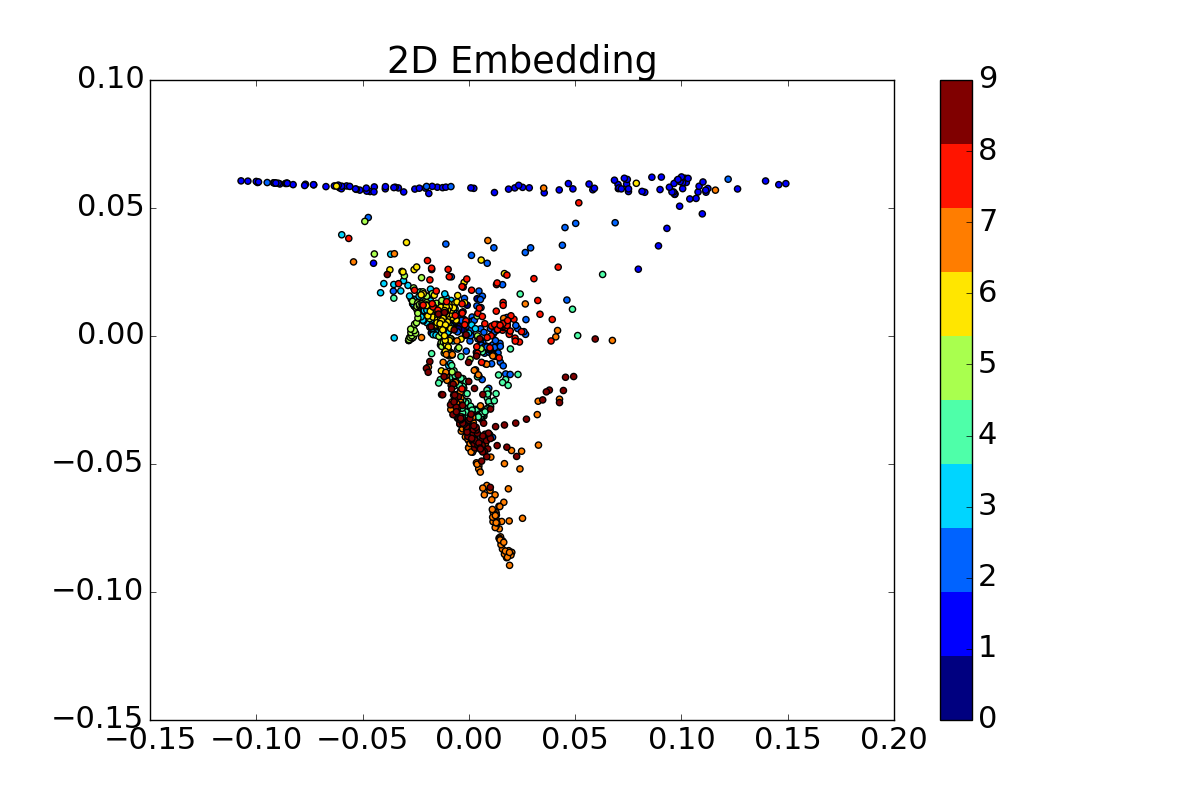
\includegraphics[width=0.5\textwidth]{plots/2dEmbedding}
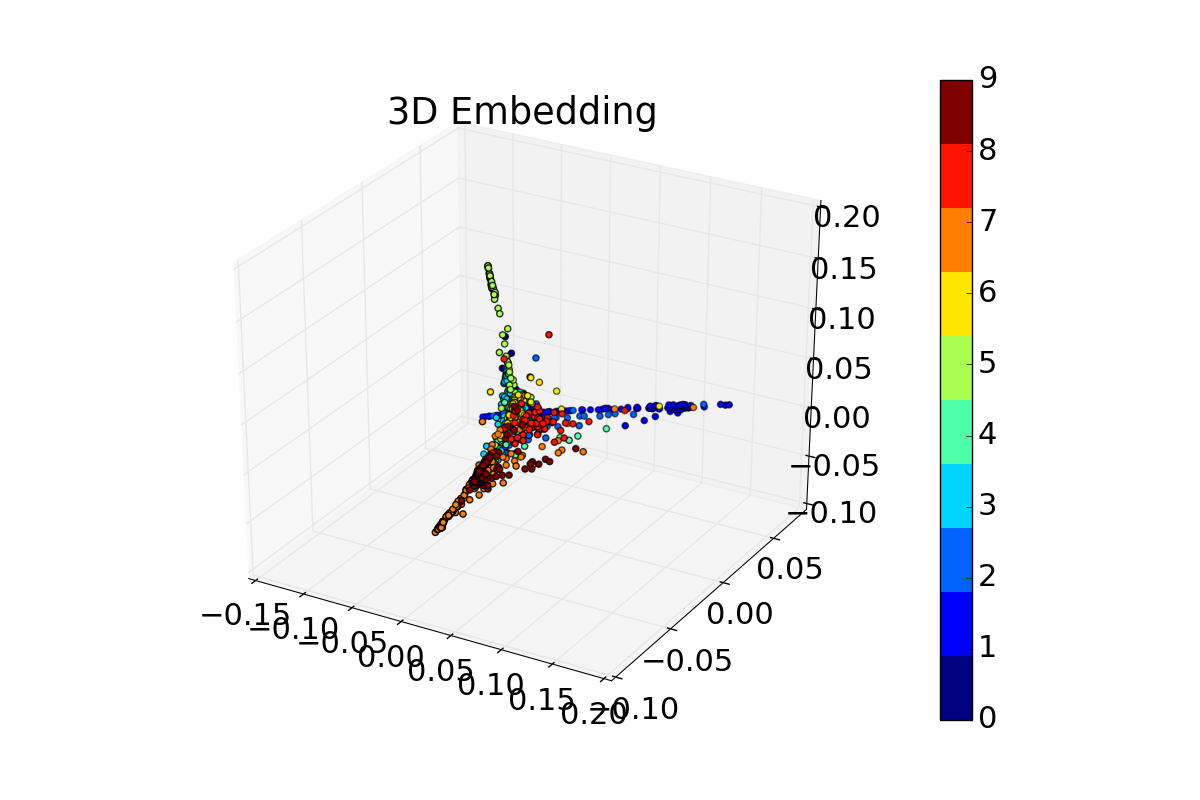
\includegraphics[width=0.5\textwidth]{plots/3dEmbedding}


c)
The matrix $M$ contains block structures which appear when the samples are sorted by their label. The neighbors of a data point are very likely to have the same label. This is why these block structures appear.

\begin{center}
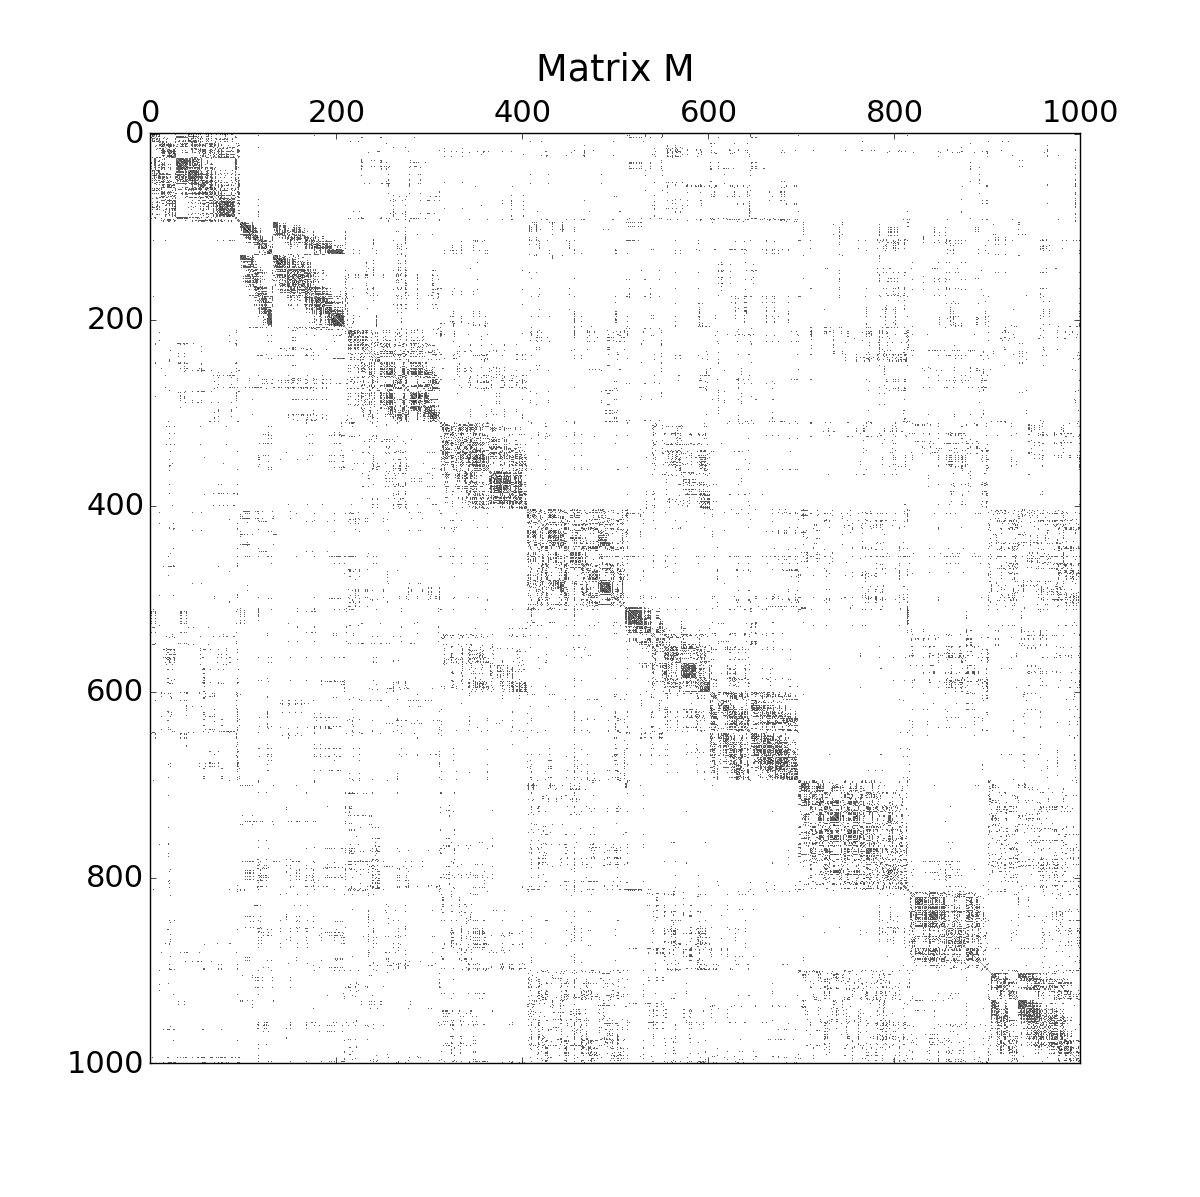
\includegraphics[width=0.4\textwidth]{plots/matrixM}
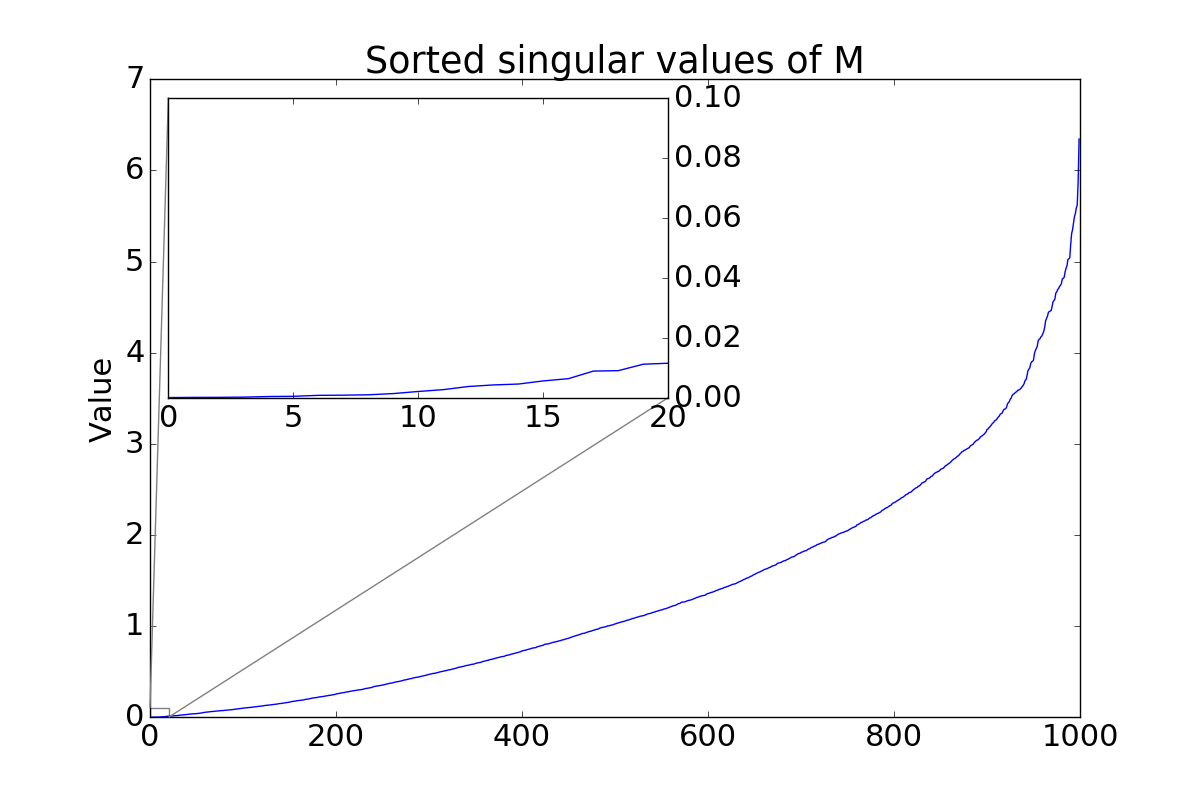
\includegraphics[width=0.5\textwidth]{plots/singularM}
\end{center}

	

Since we want to minimize the cost we are looking for the eigenvectors with the lowest eigenvalues.
The first 5 to 10 singular values are close to zero. This makes sense since we have 10 different labels. A good choice for the embedding dimension would therefore be 10 (one coordinate per label).

\begin{center}

\end{center}

}

\problemAnswer{ % Answer


d) With more neighbors the manifold is smoother. The following two figures illustrate this:

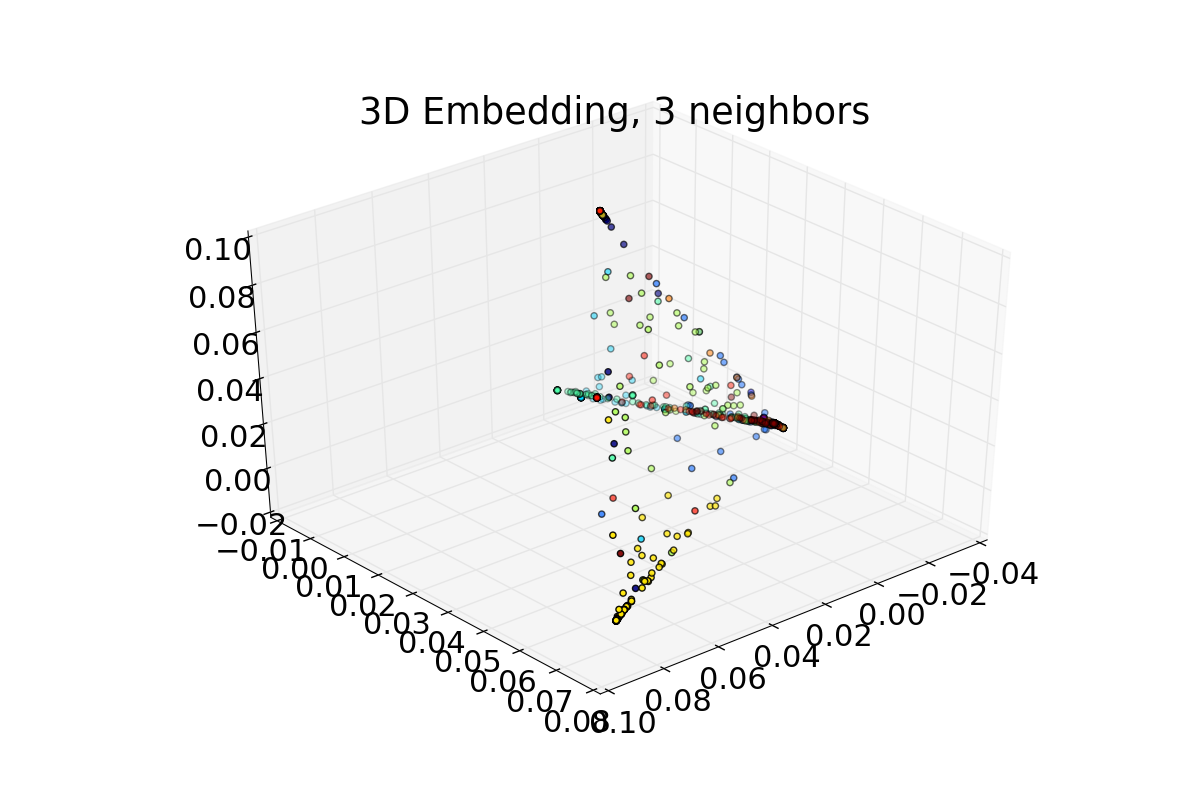
\includegraphics[width=0.5\textwidth]{plots/3d3neighbors}
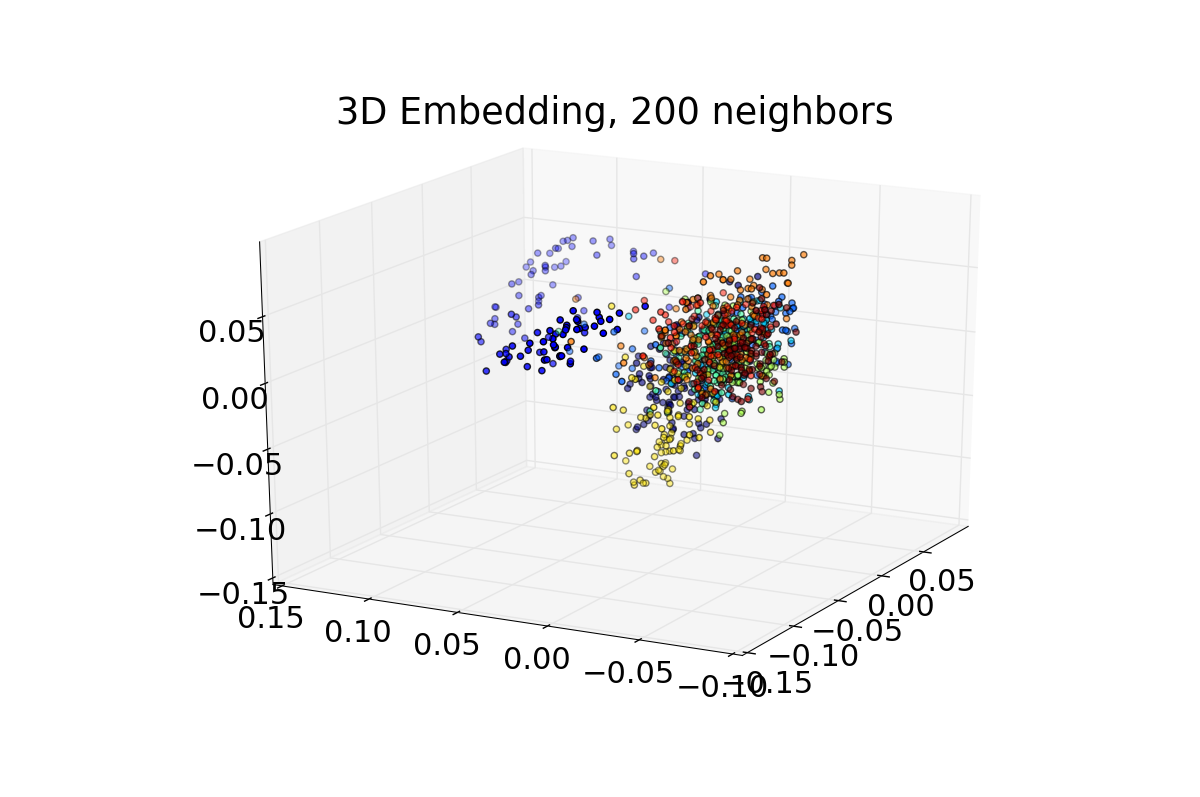
\includegraphics[width=0.5\textwidth]{plots/3d200neighbors}

I implemented another way to determine the neighbors of a datapoint. Since we are dealing with images I use the structural similarity\footnote{https://en.wikipedia.org/wiki/Structural\_similarity} on the smoothed images (Gaussian filter with $\sigma=1$). The resulting matrix $M$ is slightly better diagonalized (less neighbors with different labels). See appendix for figures.

\vspace*{1em}
e) As a first attempt I tried to mimic a reversal of the embedding. I determined the closest neighbors of a point in the embedded space and then assigned weights to these neighbors, so that the linear combination results in the chosen point (number of neighbors equals the dimension of the embedded space). Then I simply computed the weighted average of the high dimensional neighbors. The results are not satisfactory and this method only works if the point is very close to an already existing one. See gif at \emph{/plots/interpolation2d.gif}.

A more promising method is to learn the mapping with machine learning. 
Kernelized ridge regression with a linear kernel worked surprisingly well. Other regression methods either just interpolate between the two high dimensional pictures or only learn an average representation (which they then predicted for all inputs).
I set the dimension of the embedded space to 30 and increased the number of neighbors to 30 as well. This improved the reconstruction, most likely because the manifold is smoother with more neighbors, as mentioned before. The only post-processing step is to set every pixel which has a value below 0 to 0.
The following figure shows the path along which the reconstructions were computed, the gif is located at \emph{/plots/reconstruct3to7.gif} (or see appendix for a few of the intermediate stages and what happens outside of the manifold).

\begin{center}
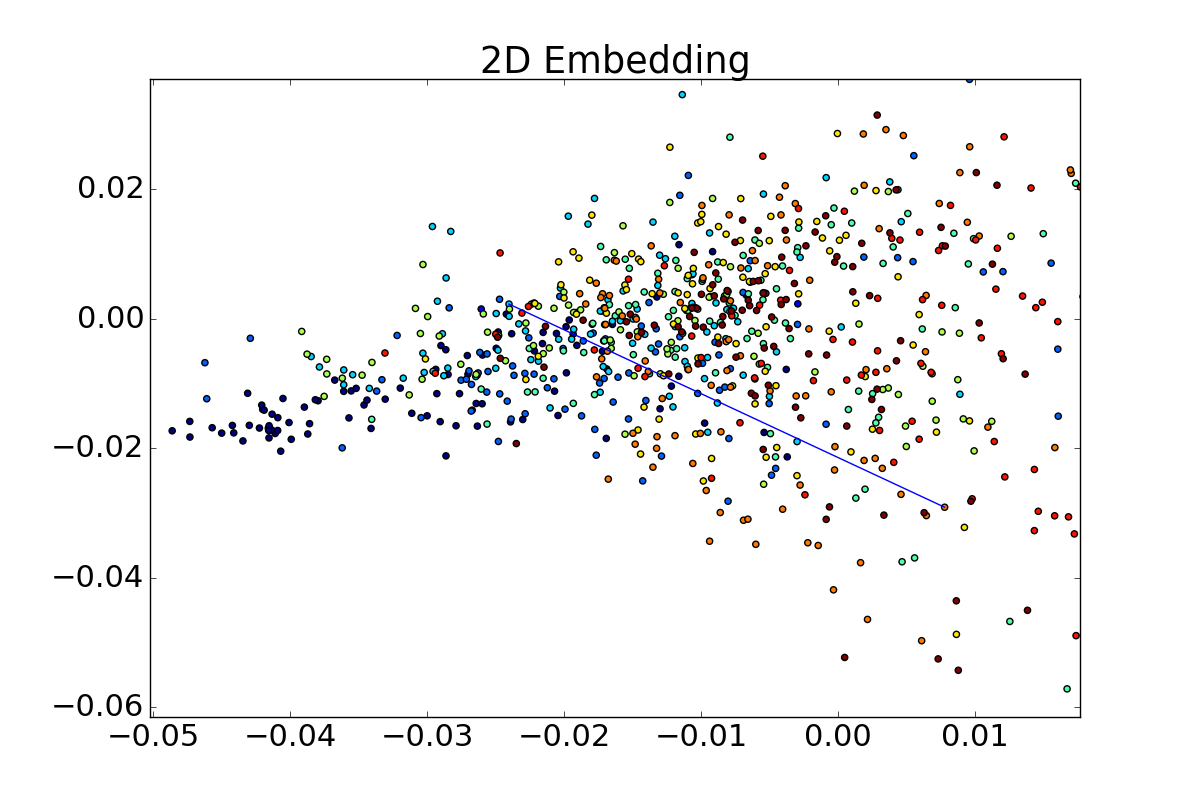
\includegraphics[width=0.5\textwidth]{plots/reconstructionPath}
\end{center}




I also tried using a neural network but it only learned an "average" high dimensional representation (see appendix).

}
\end{homeworkProblem}
\clearpage

%----------------------------------------------------------------------------------------
\begin{homeworkProblem}[The Implementation]

In the implementation section you give a concise insight to the practical aspects of this coding exercise. It mainly mentions the optimization methods used to solve the model equations. Did you encounter numerical or efficiency problems? If yes, how did you solve them?
Provide the link to your git branch of this coding exercise.\newline
Hard limit: One page

\vspace{10pt}
\problemAnswer{ % Answer
	
Branch name \hmwkGitBranch
	
The code is located at ./code/locally\_linear\_embedding.py.
\vspace*{0.5em}


\textbf{Algorithm}

	\begin{enumerate}
	\item Compute the Neighbors of each data point, $X_i$.
	\item Compute the weights $W_{ij}$ that best reconstruct each data point $X_i$ from its neighbors, minimizing the cost by constrained linear fits.
	\item Compute the vectors $Y_i$ best reconstructed by the weights $W_{ij}$ minimizing the quadratic form by its bottom nonzero eigenvectors.
\end{enumerate}

The weights in step 2 can be computed by solving the following linear system of equations

\[
\sum_j C_{jk}w_k = 1
\]

and then rescaling the weights so that they sum to one for each data point.

\vspace*{1em}

\textbf{Implementation}

The MNIST loading code is taken from 

https://github.com/sorki/python-mnist/blob/master/mnist/loader.py.
\vspace*{0.5em}

The implementation of the LLE algorithm was done mostly from scratch with occasional comparison to the implementation of the sci-kit learn module

(https://github.com/scikit-learn/scikit-learn/blob/14031f6/sklearn/manifold/locally\_linear.py\#L508)

and the Matlab code provided here: https://www.cs.nyu.edu/$\sim$roweis/lle/code.html.

\vspace*{1em}
The implementation works with a sparse csr matrix and uses the arpack \texttt{eigsh} function to solve for the eigenvectors. 
I never encountered performance problems with this implementation (See figure below for performance).
Numerical instabilities are prevented by adding a small value to the main diagonal of the covariance matrix (as proposed in the paper\footnote{"An Introduction to Locally Linear Embedding" by L. Saul and S. Roweis}, appendix A equation 6).

The hardest part of the implementation was at first understanding which steps were actually required for the algorithm and then to have the correct shapes, dimensions and transpositions for the matrices and vectors.

The performance of the algorithm is a bit slower than $O(n^2)$.

\begin{center}
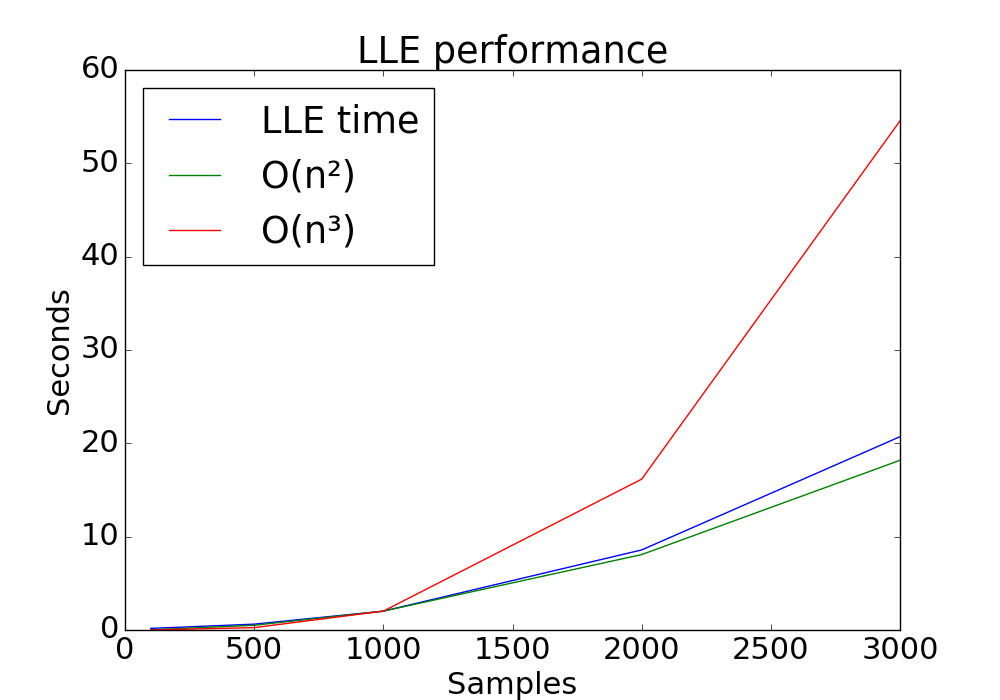
\includegraphics[width=0.5\textwidth]{plots/LLEperformance}
\end{center}

}
\end{homeworkProblem}
\clearpage

%----------------------------------------------------------------------------------------
\begin{homeworkProblem}[Your Page]
Your page gives you space to include ideas, observations and results which do not fall into the categories provided by us. You can also use it as an appendix to include things which did not have space in the other sections.\newline
No page limit.

\vspace{10pt}
\problemAnswer{ % Answer

\hmwkGitBranch % defined in line 5


\textbf{Comparison of different neighbor methods}

The matrix on the left was constructed with neighbors determined by Euclidean distance. The matrix on the right by the structural similarity (SSIM) of the images. SSIM leads to a slightly better diagonalized matrix (check column 400 to 500).

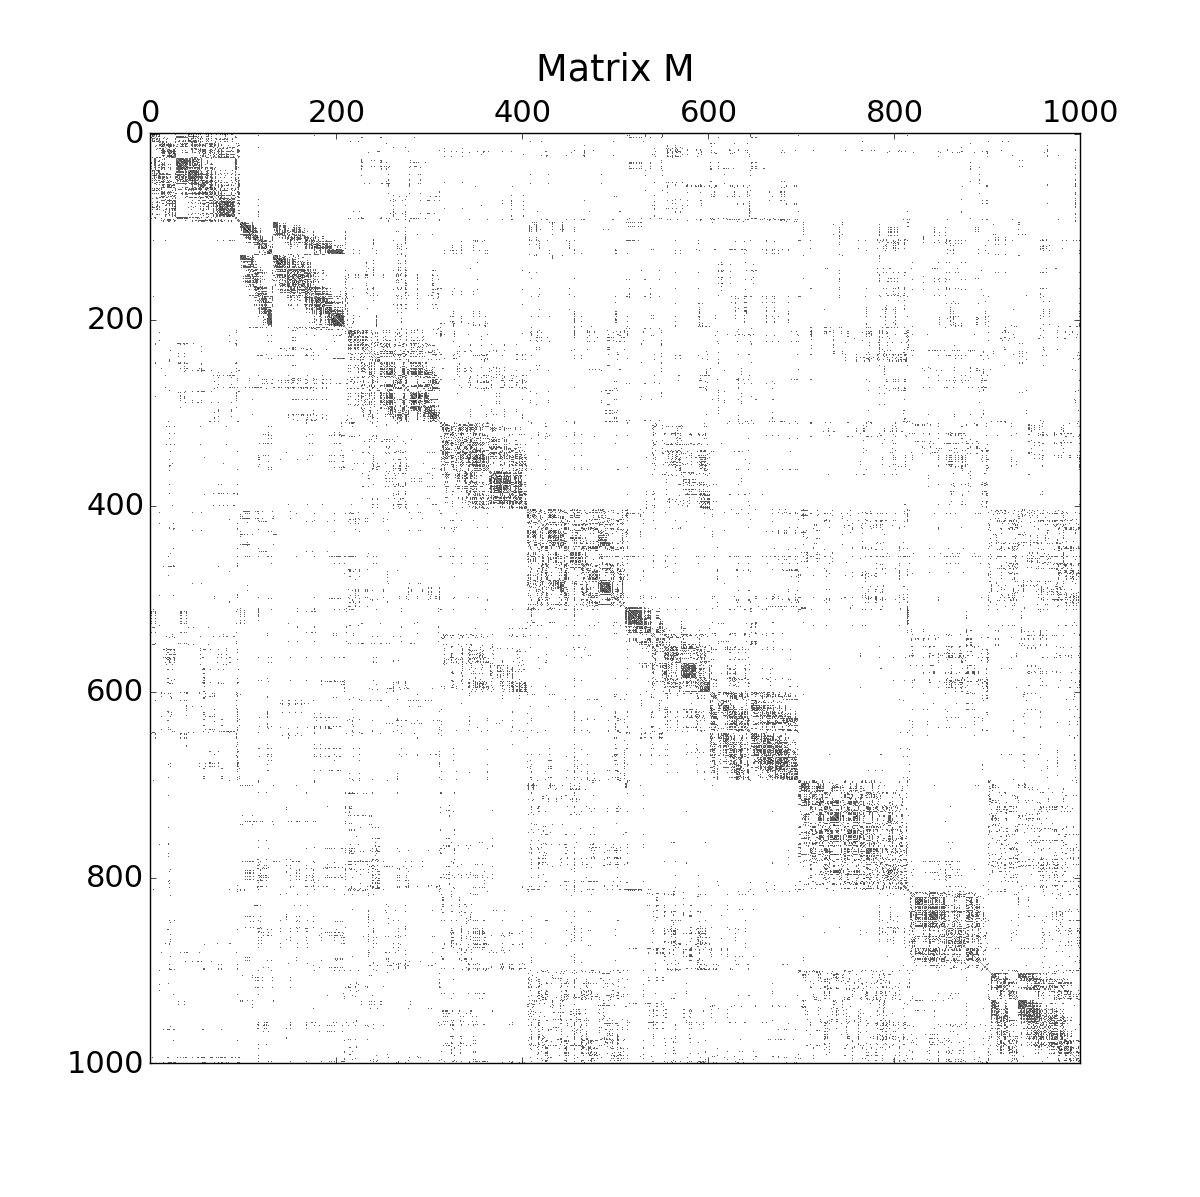
\includegraphics[width=0.4\textwidth]{plots/matrixM}
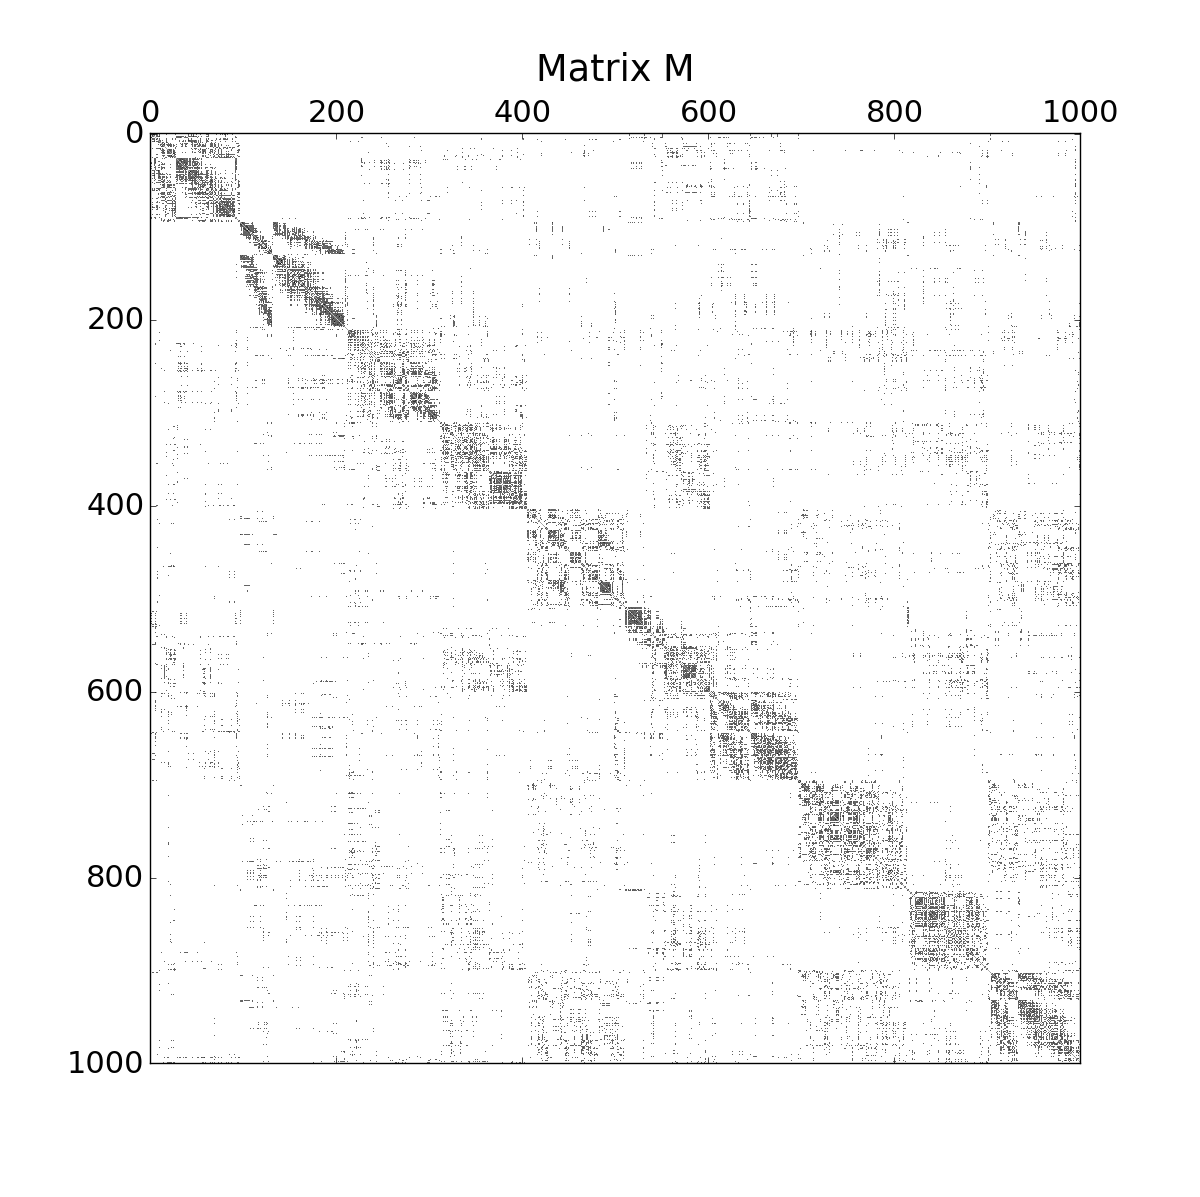
\includegraphics[width=0.4\textwidth]{plots/ssimMatrixM}


The resulting embeddings are quite similar, except for a rotation. (Left Euclidean distance, right SSIM)

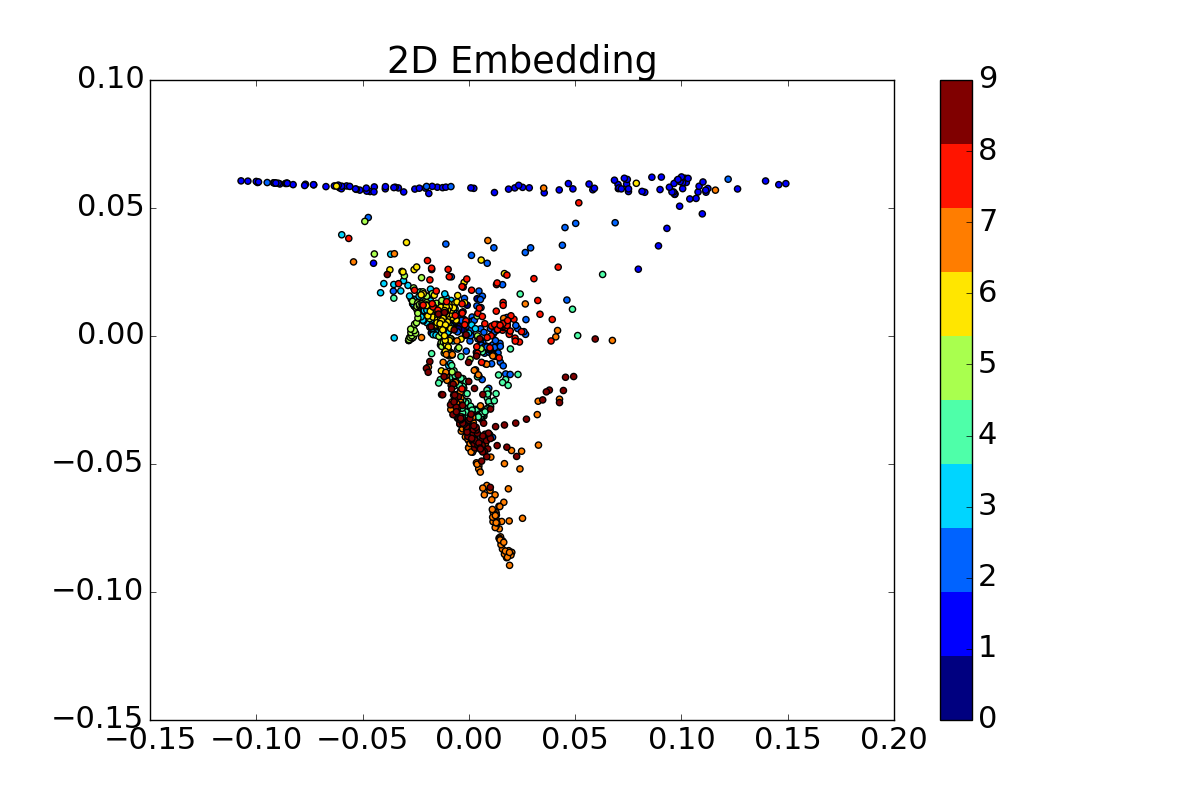
\includegraphics[width=0.5\textwidth]{plots/2dEmbedding}
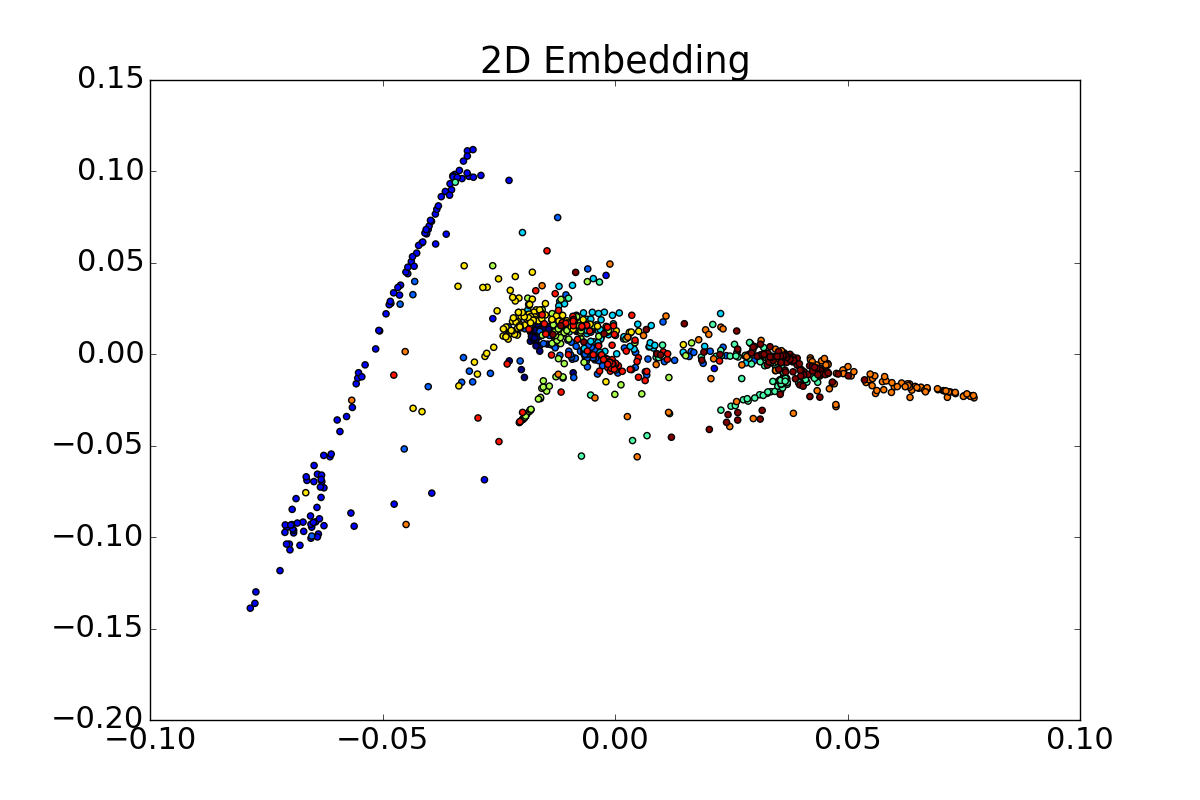
\includegraphics[width=0.5\textwidth]{plots/ssim2dEmbedding}



\textbf{Learning the reverse mapping}

The kernelized ridge regression learned to reconstruct arbitrary points on the manifold. The following pictures are some of the stages contained in the reconstruction gif (\emph{/plots/reconstruct3to7.gif}).

\begin{center}
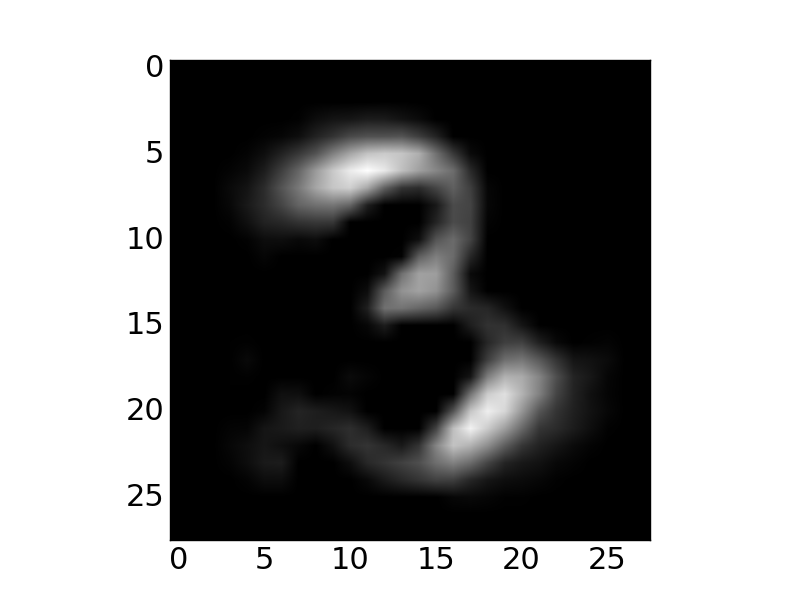
\includegraphics[width=0.2\textwidth]{plots/reconstruct_0}
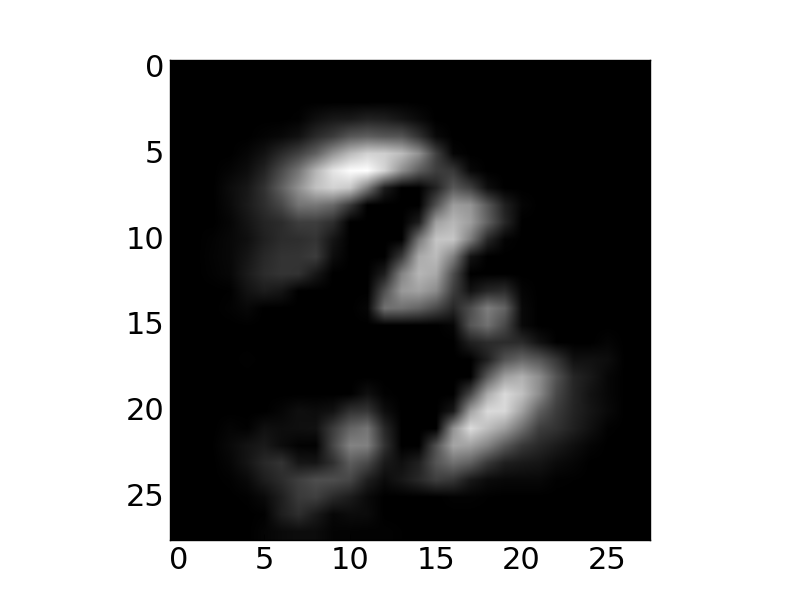
\includegraphics[width=0.2\textwidth]{plots/reconstruct_3}
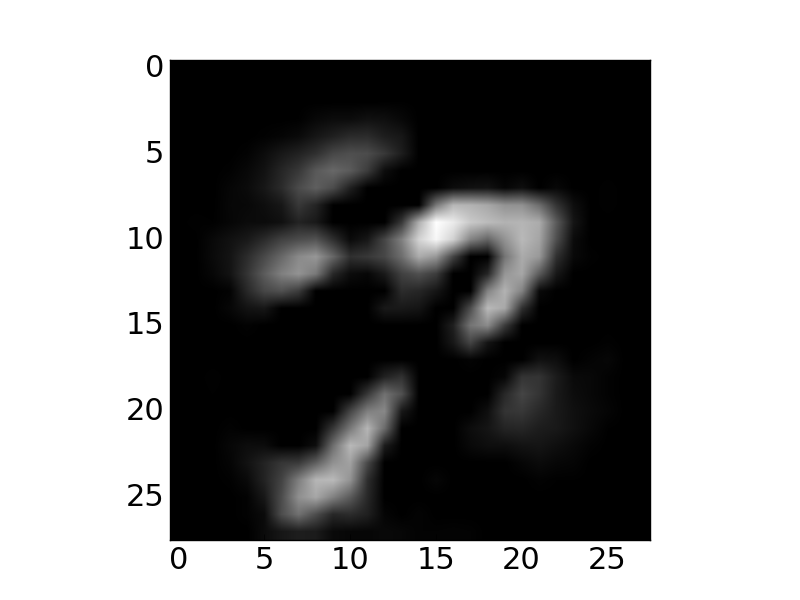
\includegraphics[width=0.2\textwidth]{plots/reconstruct_6}
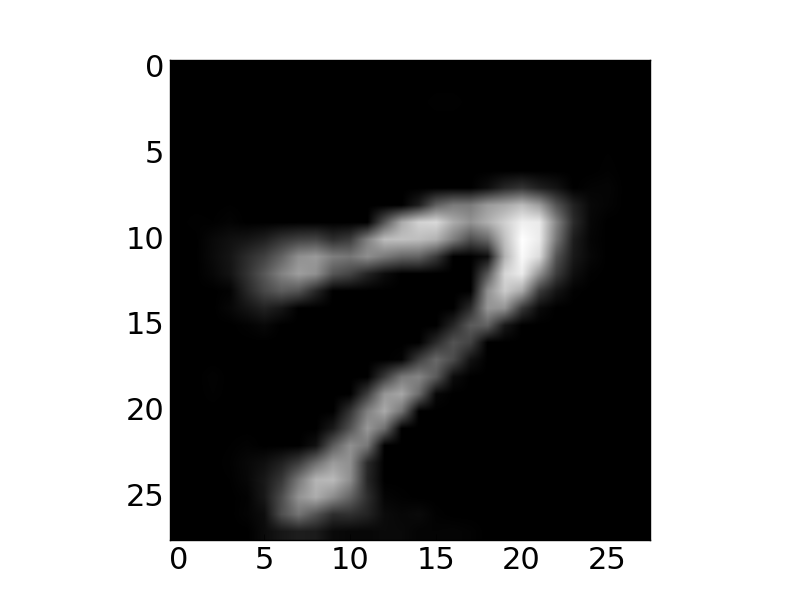
\includegraphics[width=0.2\textwidth]{plots/reconstruct_10}
\end{center}

}

\problemAnswer{ % Answer

Outside of the manifold the reconstructions do no longer clearly represent a digit. But they still have some features of the digits (certain curves etc.).

\begin{center}
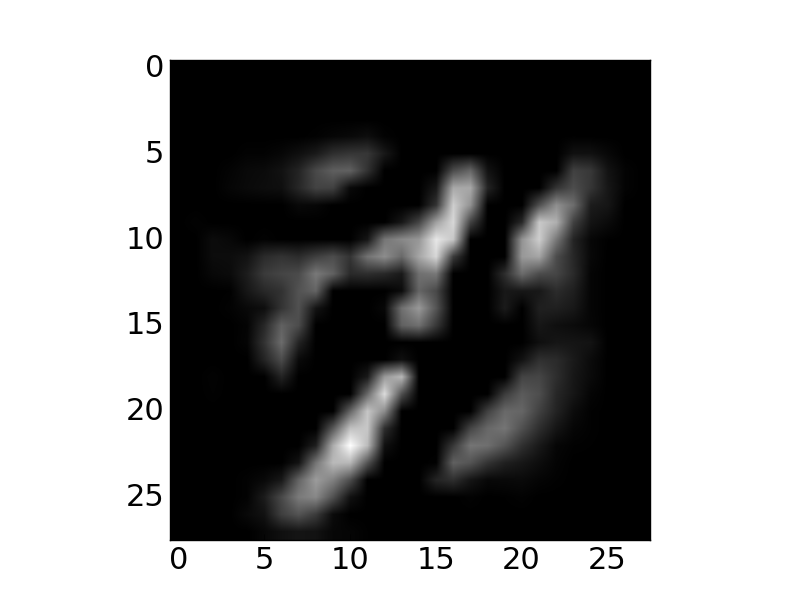
\includegraphics[width=0.5\textwidth]{plots/outsideManifold}
\end{center}

The neural network mentioned in task (e) had learned the following "average" high dimensional representation. The network returned this for all inputs (with small deviations).


\begin{center}
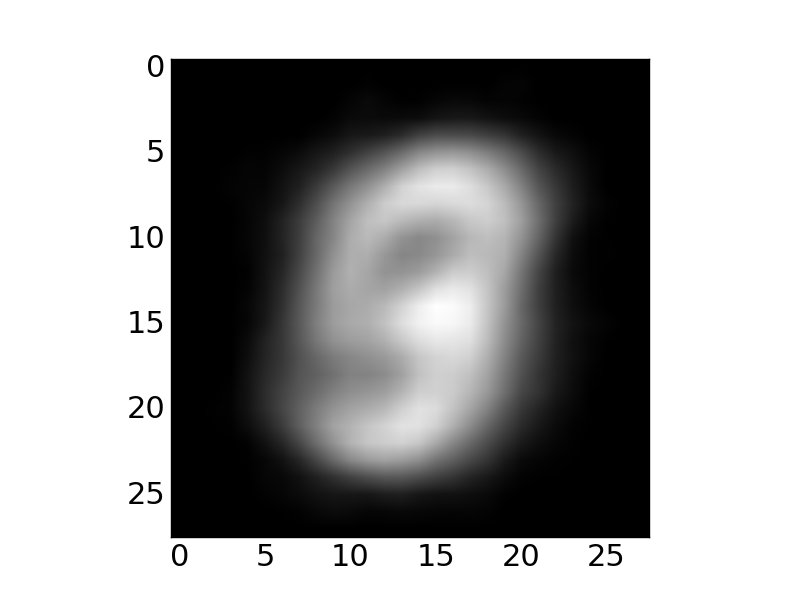
\includegraphics[width=0.5\textwidth]{plots/learnedMappingNN}
\end{center}

}
\end{homeworkProblem}
\clearpage

\end{document}

